\documentclass[12pt]{article}

\usepackage{amsmath}
\usepackage{amssymb}
\usepackage{amsthm}

\usepackage{graphicx}
\graphicspath{ {./} }

\usepackage[utf8]{inputenc}
\usepackage[T1]{fontenc}

\usepackage[inline]{enumitem}

\newtheorem{theorem}{Theorem}
\newtheorem{lemma}{Lemma}
\newtheorem*{prop}{Proposition}
\newtheorem{definition}{Definition}
\newtheorem*{example}{Example}
\newtheorem*{notation}{Notation}

\begin{document}

\title{Rational Parking Functions}
\author{Matthieu Josuat-Vergès \and Tessa Lelièvre-Osswald}
\date{August 27, 2020}

\maketitle

\begin{abstract}
    This is an abstract about Rational Parking Functions
\end{abstract}

\begin{displaymath}
\end{displaymath}

\section{Parking Functions}

\begin{definition}[Parking Function]
    A \emph{parking function} is a sequence $(a_1, a_2, \ldots, a_n)$
    such that its non-decreasing reordering $(b_1, b_2, \ldots, b_n)$
    has $b_i < i$ for all $i$.\\
    We denote by $\mathcal{PF}_n$ the set of parking functions of length $n$.
    $$\mathcal{PF} = \bigcup_{n > 0}{\mathcal{PF}_n}$$.
\end{definition}

\begin{example}
    \begin{align*}
    &f_1 = (7, 3, 1, 4, 2, 5, 2) \in \mathcal{PF}_7\\
    &f_2 = (7, 3, 1, 4, 2, 5, 4) \notin \mathcal{PF}_7\\
    \end{align*}
\end{example}

\begin{prop}
    Let $pf_n$ be the cardinal of $\mathcal{PF}_n$.
    We have $pf_n = (n + 1)^{n-1}$.
\end{prop}

\begin{example}[$n = 1, 2, 3$]
    \text{} \\
    \begin{itemize*}
            \item $n = 1$ \text{ } $:$ \text{ } $pf_1 = 1$\\
            \subitem $(1)$\\
            \item $n = 2$ \text{ } $:$ \text{ } $pf_2 = 3$\\
            \subitem $(1, 1)$
            \subitem $(1, 2)$
            \subitem $(2, 1)$\\
            \item $n = 3$ \text{ } $:$ \text{ } $pf_3 = 16$\\
            \subitem $(1, 1, 1)$
            \subitem $(1, 1, 2)$
            \subitem $(1, 1, 3)$
            \subitem $(1, 2, 1)$
            \subitem $(1, 2, 2)$
            \subitem $(1, 2, 3)$
            \subitem $(1, 3, 1)$
            \subitem $(1, 3, 2)$
            \subitem $(2, 1, 1)$
            \subitem $(2, 1, 2)$
            \subitem $(2, 1, 3)$
            \subitem $(2, 2, 1)$
            \subitem $(2, 3, 1)$
            \subitem $(3, 1, 1)$
            \subitem $(3, 1, 2)$
            \subitem $(3, 2, 1)$\\
    \end{itemize*}
\end{example}

\begin{definition}[Primitive]
    A parking function $(a_1, a_2, \ldots, a_n)$ is said \emph{primitive} if
    it is already in non-decreasing order. \\
    We denote by $\mathcal{PPF}_n$ the set of primitive parking functions of length $n$.
    $$\mathcal{PPF} = \bigcup_{n > 0}{\mathcal{PPF}_n}$$
    
\end{definition}

\begin{example}
    \begin{align*}
        &f_1 = (1, 2, 2, 3) \in \mathcal{PPF}_4\\
        &f_2 = (1, 2, 3, 2) \notin \mathcal{PPF}_4
         \text{, even though } f_2 \in \mathcal{PF}_4\\
    \end{align*}
\end{example}

\begin{prop}
    Let $ppf_n$ be the cardinal of $\mathcal{PPF}_n$.
    We have $ppf_n = \frac{1}{n + 1} \binom{2n}{n}$,
    which is the $n^{th}$ Catalan number.
\end{prop}

\begin{example}[$n = 1, 2, 3$]
    \text{}\\
    \begin{itemize*}
        \item $n = 1$ \text{ } $:$ \text{ } $ppf_1 = 1$\\
        \subitem $(1)$\\
        \item $n = 2$ \text{ } $:$ \text{ } $ppf_2 = 2$\\
        \subitem $(1, 1)$
        \subitem $(1, 2)$\\
        \item $n = 3$ \text{ } $:$ \text{ } $ppf_3 = 5$\\
        \subitem $(1, 1, 1)$
        \subitem $(1, 1, 2)$
        \subitem $(1, 1, 3)$
        \subitem $(1, 2, 2)$
        \subitem $(1, 2, 3)$\\
    \end{itemize*}
\end{example}

\section{Non-crossing Partitions}

\begin{definition}[Non-crossing Partition]
    A \emph{non-crossing partition} of a set $E$ is
    a set partition $P = \{E_1, E_2, \ldots, E_k\}$ such that
    if $a, c \in E_i$, $b, d \in E_j$, and $i \neq j$, then
    we do \emph{not} have $a < b < c < d$, nor $a > b > c > d$.\\
    We denote by $\mathcal{NC}_n$ the set of non-crossing partitions
    of $\{1, 2, \ldots, n\}$.
    $$\mathcal{NC} = \bigcup_{n > 0}{\mathcal{NC}_n}$$
\end{definition}

\begin{notation}
    $[n] = \{1, 2, \ldots, n\}$
\end{notation}

\begin{example}[$E = \lbrack 6 \rbrack $]
    \begin{align*}
        &P_1 = \{\{1, 2, 5\}, \{3, 4\}, \{6\}\} \in \mathcal{NC}_6\\
        &P_2 = \{\{1, 2, 4\}, \{3, 5\}, \{6\}\} \notin \mathcal{NC}_6
    \end{align*}
\end{example}

\begin{prop}
    Let $nc_n$ be the cardinal of $\mathcal{NC}_n$.
    We have $nc_n = \frac{1}{n + 1} \binom{2n}{n}$,
    which is the $n^{th}$ Catalan number.
\end{prop}

\begin{example}[$n = 1, 2, 3$]
    \text{}\\
    \begin{itemize*}
        \item $n = 1$ \text{ } $:$ \text{ } $nc_1 = 1$\\
        \subitem $\{\{1\}\}$\\
        \item $n = 2$ \text{ } $:$ \text{ } $nc_2 = 2$\\
        \subitem $\{\{1, 2\}\}$
        \subitem $\{\{1\}, \{2\}\}$\\
        \item $n = 3$ \text{ } $:$ \text{ } $nc_3 = 5$\\
        \subitem $\{\{1, 2, 3\}\}$
        \subitem $\{\{1\}, \{2, 3\}\}$
        \subitem $\{\{1, 3\}, \{2\}\}$
        \subitem $\{\{1, 2\}, \{3\}\}$
        \subitem $\{\{1\}, \{2\}, \{3\}\}$\\
    \end{itemize*}
\end{example}

\begin{prop}
    This means we can create a \emph{bijection} between
    $\mathcal{PPF}_n$ and $\mathcal{NC}_n$.
\end{prop}

\begin{itemize}
    \item $\mathcal{NC}_n \to \mathcal{PPF}_n$ :
    For each block $B$ in the non-crossing partition, take
    $i = min (B)$, and $k_i = size (B)$.\\
    $k_i = 0$ if $i$ is not the minimum of a block.\\
    The corresponding parking function is
    $(\underbrace{1, \ldots, 1}_{k_1}, \underbrace{2, \ldots,
    2}_{k_2}, \ldots, \underbrace{n, \ldots, n}_{k_n})$.\\
    \item $\mathcal{PPF}_n \to \mathcal{NC}_n$ :
    For each $i$ in $[n]$, if $i$ appears $n_i$ times in the
    parking function, $B_i$ will be of size $n_i$ with minimum
    element $i$.
    There is a unique set partition $\displaystyle P = \bigcup_{i}{B_i}$
    of $[n]$ respecting these conditions that is non-crossing.
\end{itemize}

\begin{example}[$E = \lbrack 6 \rbrack$]
    \begin{align*}
        &P = \{\{1, 2, 5\}, \{3, 4\}, \{6\}\}
        &f = (1, 1, 1, 3, 3, 6)\\
    \end{align*}
\end{example}

A non-crossing partition of $[n]$ can be represented graphically
on a regular $n$-vertices polygon, with vertices labeled from $1$
to $n$ clockwise. We then represent each block $B = \{b_1, \ldots, b_k\}$
by the convex hull of $\{b_1, \ldots, b_k\}$.

\begin{example}[$P = \{\{1, 2, 5\}, \{3, 4\}, \{6\}\}$]
    \text {}\\
    \begin{align*}
    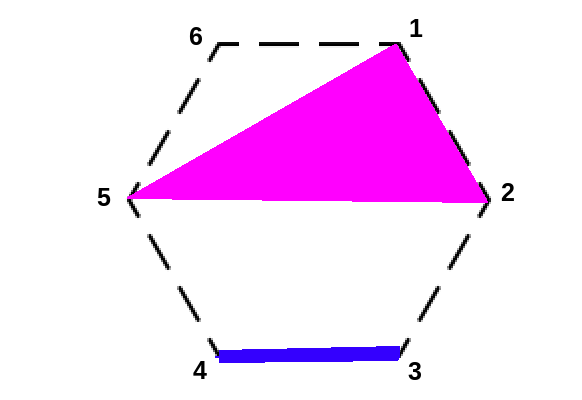
\includegraphics[scale = 0.3]{fig2}
    \end{align*}
\end{example}

Thus non-crossing meaning the hulls are \emph{disjoint}.

\end{document}